
\subsection{Inverse dynamics}
The objective of this activity is display the UR5 robot on rviz and control the motion of its joints with inverse dynamics control method. The simulation starts with the initial joint configuration $\begin{bmatrix} \pi & -\frac{\pi}{8} & -\frac{\pi}{6} & 0.0 & 0.0 & 0.0 \end{bmatrix}$ rad and then move the second and fifth joints of the UR5 robot. The two joints will move following a sinusoidal trajectory during the first 4 seconds and maintain a constant joint position during the last second. Finally, the rosnode file that control the movement of the six joints of UR5 robot is described in Algorithm \ref{lst:inverse_dynamics_control}. In this file, the inverse dynamics is configure with $K_p=600$ $\mathrm{\frac{N.m}{rad}}$ and $K_d=30$ $\mathrm{\frac{N.m.s}{rad}}$. 

Figure \ref{fig:act_2.1_joint_position} and \ref{fig:act_2.1_joint_velocity} show trajectory tracking performance of each joint of the UR5 robot. On one  hand, second and fifth joints presents and excellent position tracking except when the reference trajectory change from sinusoidal to constant value. On the other hand, second and fifth joints presents velocity error at the beginning due to reference speed starting with a value other than 0.

\begin{lstlisting}[language=Python,caption={Move the second and fifth joint of UR5 robot with the required movement of activity 2.1.}, label={lst:inverse_dynamics_control}]
# =========================
#   Configuration of node
# =========================
# create a node: 
rospy.init_node("node_inverse_dynamics_control")

# public in topic /joint_states	to send joint data	
pub = rospy.Publisher('joint_states', JointState, queue_size=1000)

# loop rate (in Hz)
rate 	= rospy.Rate(1000)		# 100 [Hz]
dt 		= 1e-3					# 10  [ms]

# object(message) type JointState
jstate = JointState()

# ==========================================
#   Set initial joint configuration of UR5
# ==========================================
# initial configuration: position, velocity and acceleration 
q0 =   np.array([np.pi, -np.pi/8,  -np.pi/6, 0.0, 0.0, 0.0])
dq0 =  np.array([0.0, 0.0, 0.0, 0.0, 0.0, 0.0]) 
ddq0 = np.array([0.0, 0.0, 0.0, 0.0, 0.0, 0.0]) 

# desired trajectory: position, velocity and acceleration
q_des =   np.array([np.pi, -np.pi/8,  -np.pi/6, 0.0, 0.0, 0.0]) 
dq_des =  np.array([0.0, 0.0, 0.0, 0.0, 0.0, 0.0]) 
ddq_des = np.array([0.0, 0.0, 0.0, 0.0, 0.0, 0.0]) 

# measured trajectory: position, velocity and acceleration
q =   np.array([np.pi, -np.pi/8,  -np.pi/6, 0.0, 0.0, 0.0])
dq =  np.array([0.0, 0.0, 0.0, 0.0, 0.0, 0.0]) 
ddq = np.array([0.0, 0.0, 0.0, 0.0, 0.0, 0.0]) 

# ===========================
#   UR5 robot configuration
# ===========================
# joints name of UR5 robot
jnames = ['shoulder_pan_joint', 'shoulder_lift_joint', 'elbow_joint','wrist_1_joint', 'wrist_2_joint', 'wrist_3_joint']

# number of degress of freedom
ndof = 6
# the class robot load the ur5.urdf
ur5_robot = Robot(ndof,q0, dq0, dt)
# create inertia matrix 
M = np.zeros([ndof,ndof])
# create nonlinear effects vector
b = np.zeros(ndof)

# ===============================
#   PD controller configuration
# ===============================
# proportional gain
kp = 600*np.ones(ndof)
# derivative gain
kd = 30*np.ones(ndof)
# control vector
tau = np.zeros(ndof)    

#===============
#   Simulation
#===============
t = 0.0             # [sec] 
sim_duration = 5.0  # [sec]
sine_duration = 4.0 # [sec]

while not rospy.is_shutdown():
    # generate sinusoidal joint reference
    if t<=sine_duration:
        # second link
        q_des[1], dq_des[1], ddq_des[1] = sinusoidal_reference_generator(q0[1], dq0[1], ddq0[1], 0.2, 1, t)
        last_q_des_1 = q_des[1]
        # fifth link
        q_des[4], dq_des[4], ddq_des[4] = sinusoidal_reference_generator(q0[4], dq0[4], ddq0[4], 0.4, 1.5, t)  
        last_q_des_4 = q_des[4]  
    else:
        # second link
        q_des[1], dq_des[1], ddq_des[1] = step_reference_generator(0, last_q_des_1)
        # fifth link
        q_des[4], dq_des[4], ddq_des[4] = step_reference_generator(0 , last_q_des_4)

    # error: position and velocity
    e 	=  q_des - q
    de 	=  dq_des - dq    

    # compute inertia matrix
    M = ur5_robot.get_M()

    # compute nonlinear effects vector (b)
    b = ur5_robot.get_b()   

    # control law: PD control + Feedback linearization
    tau = M.dot(ddq_des+np.multiply(kp, e)+np.multiply(kd, de)) + b

    # send control signal
    ur5_robot.send_control_command(tau)
    # update states
    q, dq, ddq = ur5_robot.read_joint_position_velocity_acceleration()

    # publish message
    jstate.header.stamp = rospy.Time.now()
    jstate.name 		= jnames			# Joints position name
    jstate.position 	= q
    jstate.velocity 	= dq
    pub.publish(jstate)

    # update time
    t = t + dt
    # stop simulation
    if t>=sim_duration:
        print("stopping rviz ...")
        break
    rate.sleep()
\end{lstlisting}

\begin{figure}{H}
    \centering
    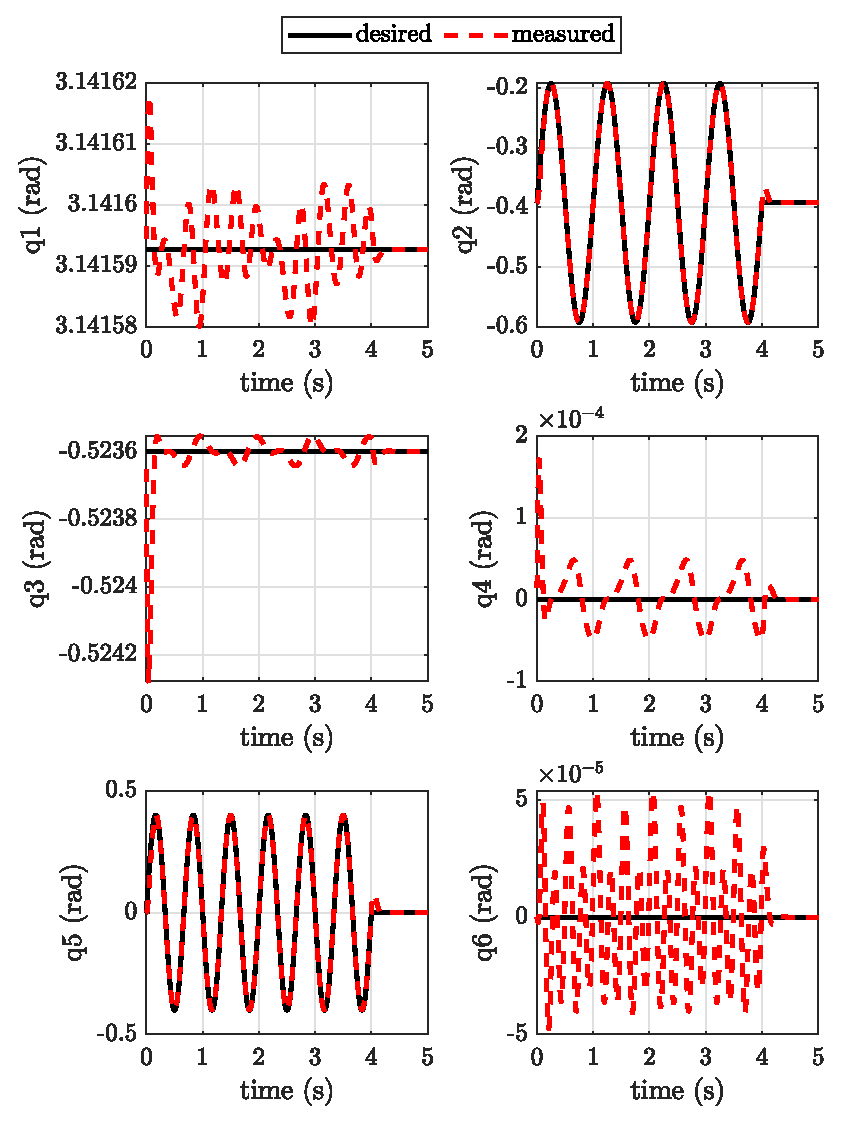
\includegraphics{images/act_2.1/joint_position.eps}
    \caption{Angular position of each joint of UR5 robot with Algorithm \ref{lst:inverse_dynamics_control}.}
    \label{fig:act_2.1_joint_position}
\end{figure}

\begin{figure}[H]
    \centering
    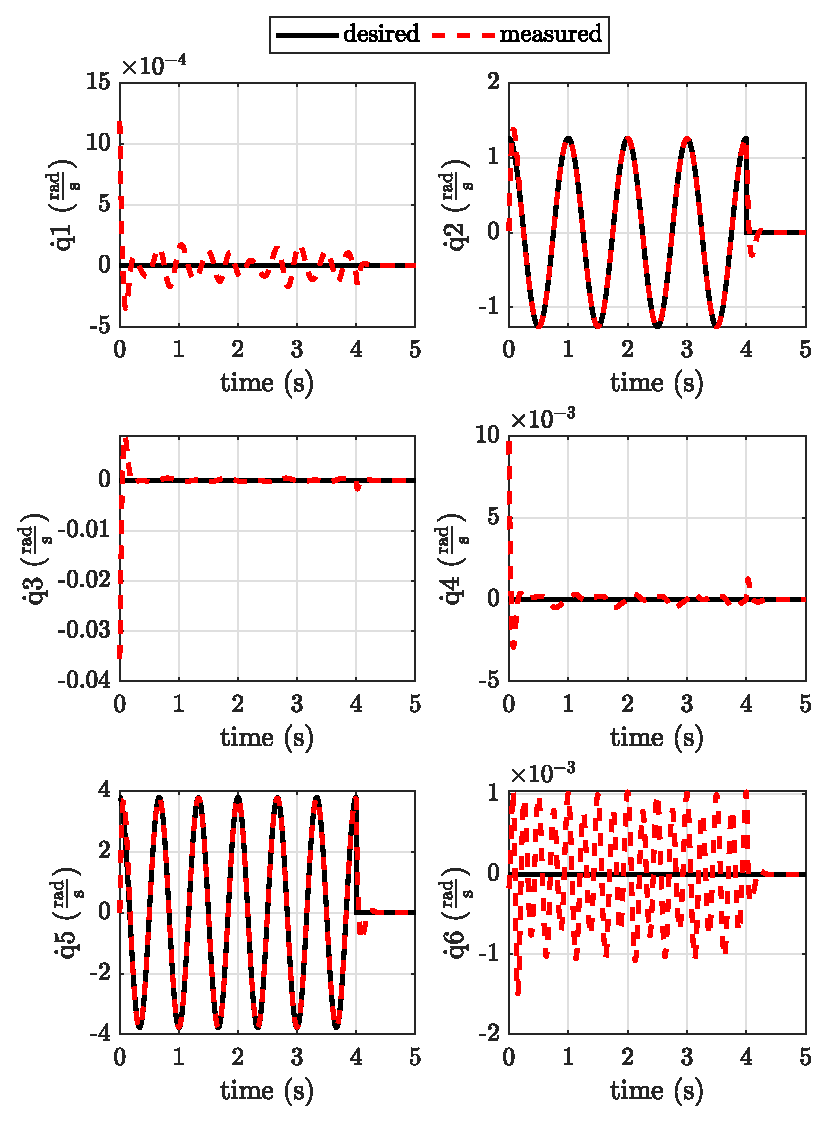
\includegraphics{images/act_2.1/joint_velocity.eps}
    \caption{Angular velocity of each joint of UR5 robot with Algorithm \ref{lst:inverse_dynamics_control}.}
    \label{fig:act_2.1_joint_velocity}
\end{figure}